\documentclass{article}
\usepackage{anuragLatexArticleStyle}
\usepackage[utf8]{inputenc}
\usepackage{bookmark}
\addbibresource{anurag.bib}

\title{Kilobotics}
\author{Anurag (183230006)\\ Eswara Srisai \\ Sudhakar Kumar (183236001) \\ Kishan}
\date{\today}

\begin{document}

\maketitle

\section{Introduction}
Kilobots (Figure \ref{fig:kilobot}) are low cost, low power, tiny robots designed by Harvard University's Self Organizing Systems Research Lab with the aim of making testing collective algorithms accesible to researchers. It has following specifications:
\begin{itemize}
	\item One IR transmitter-receiver pair
	\item One ambient light sensor
	\item Two vibrators to move robot using stick and slide mechanism
	\item One onboard battery
	\item One RGB LED
\end{itemize}
\begin{figure}[H]
	\centering
	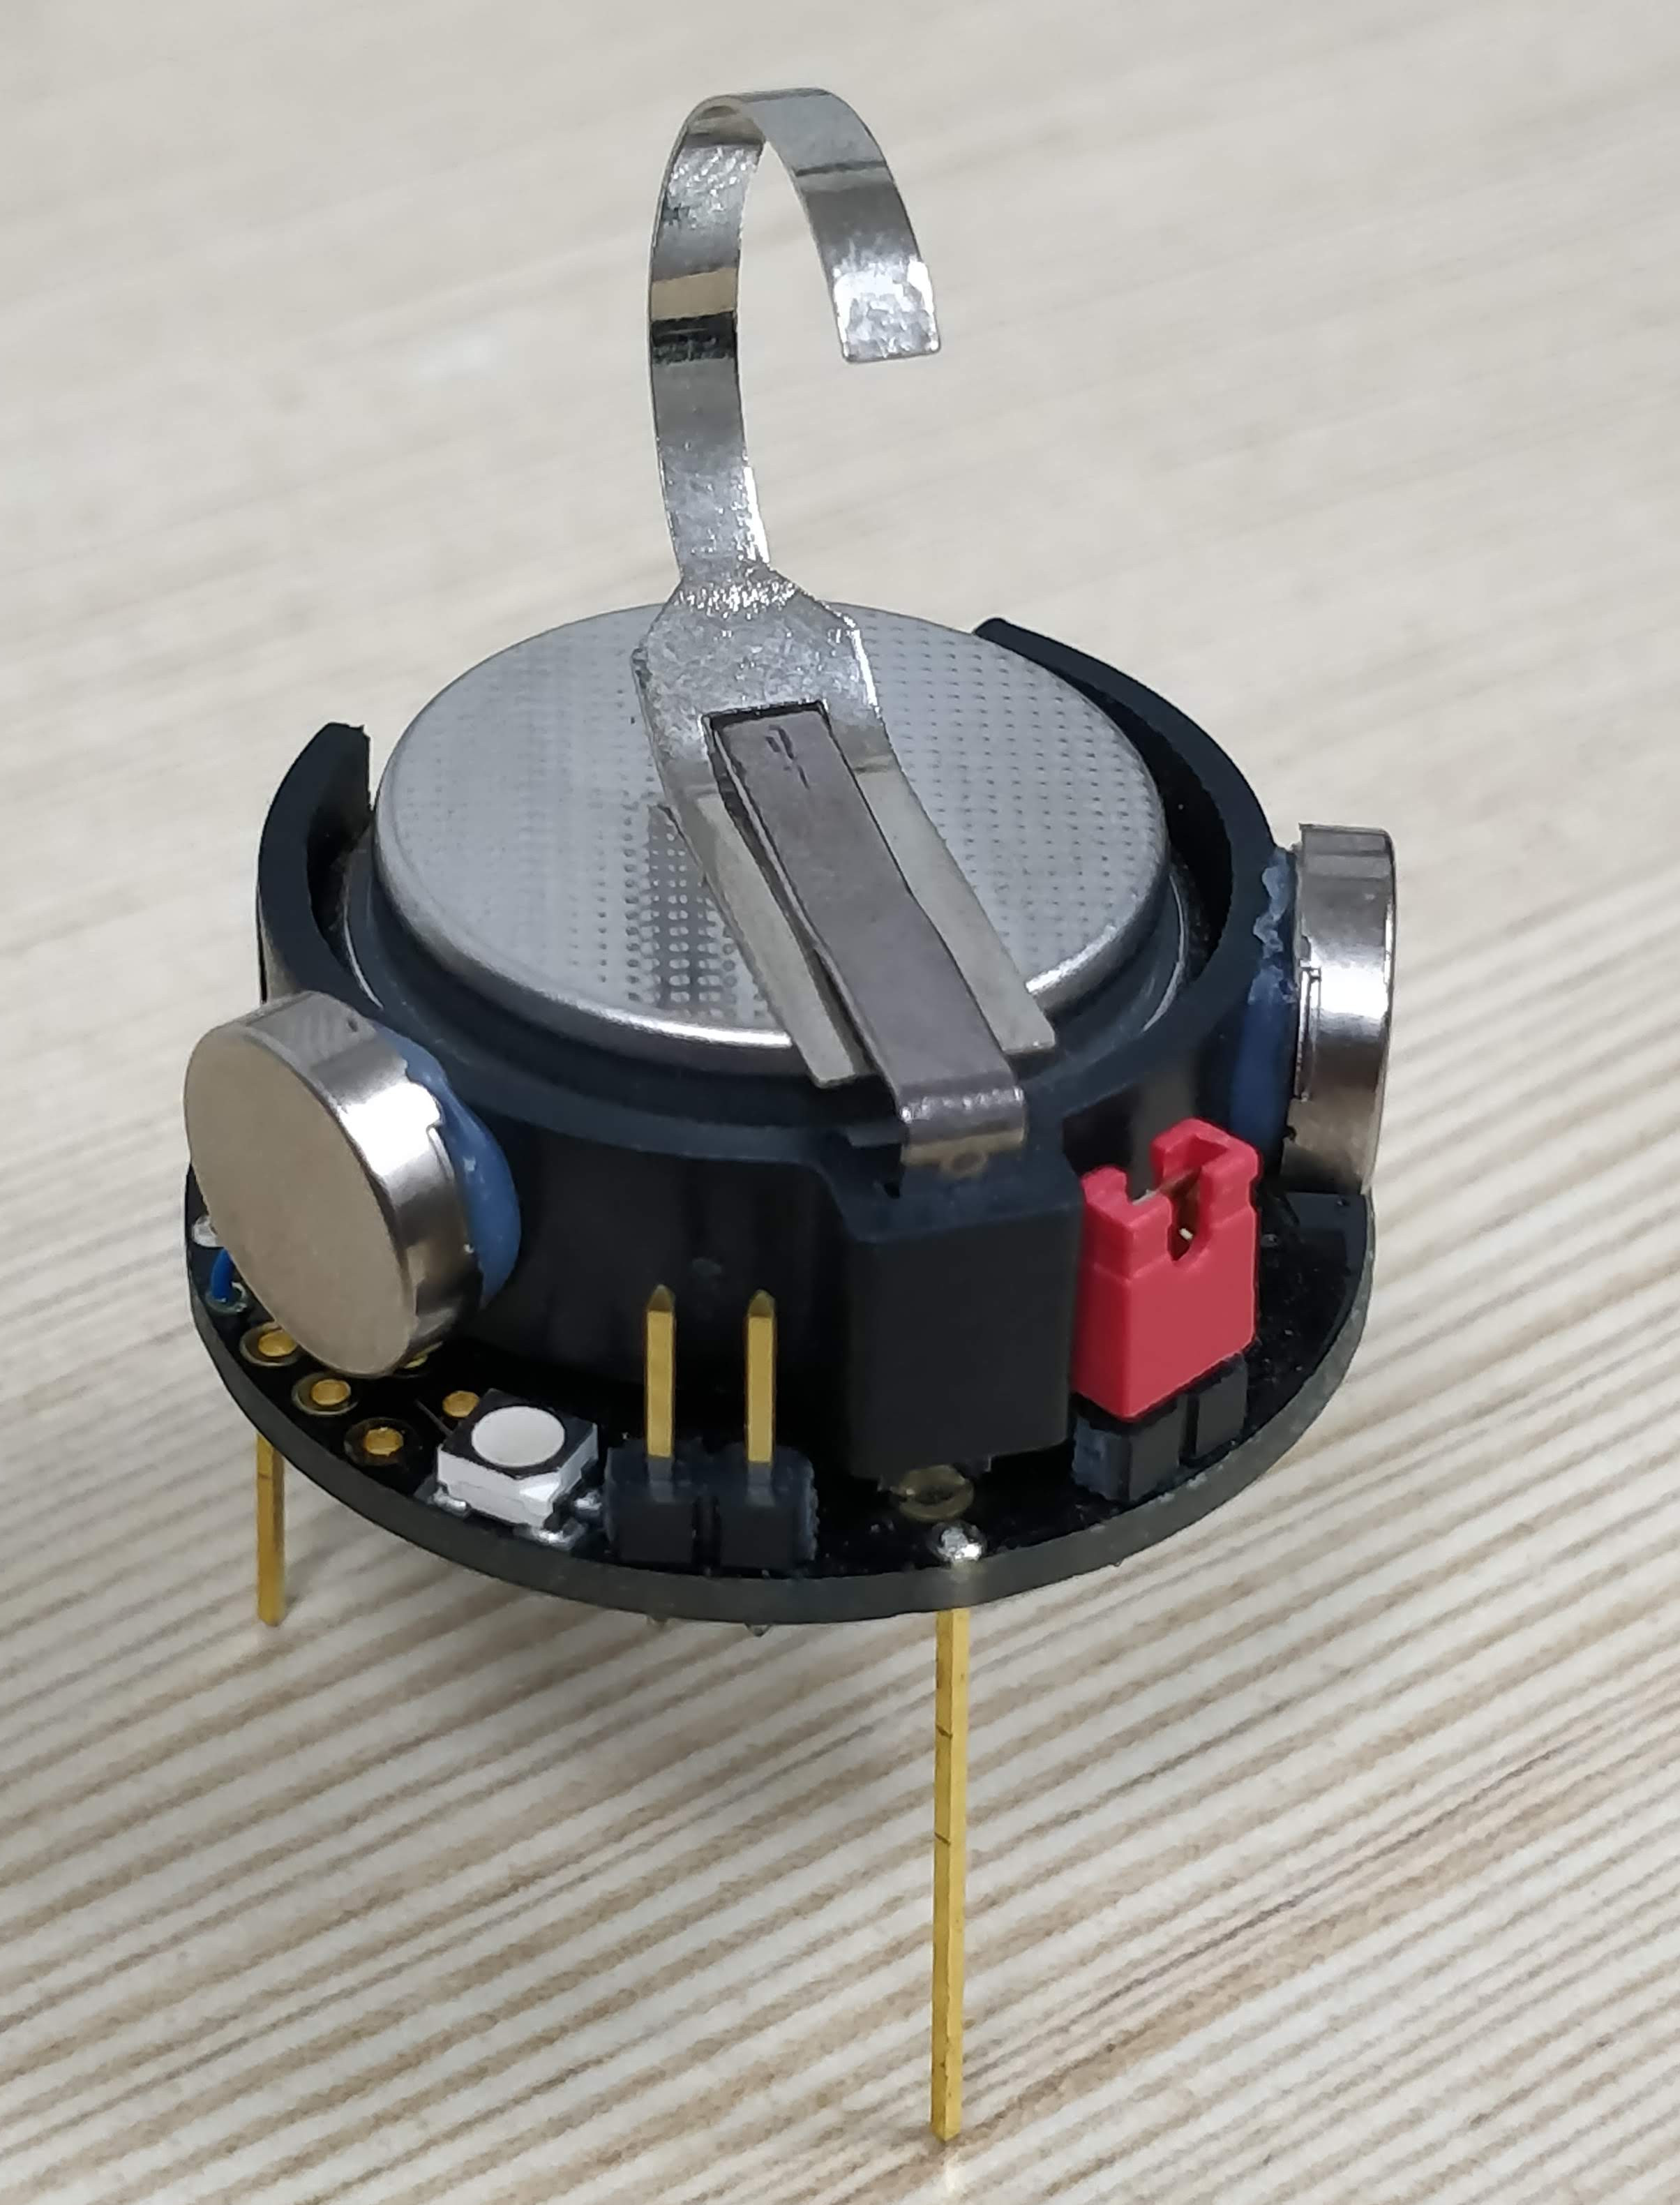
\includegraphics[scale=0.04]{images/kilobots}
	\caption{Kilobot}
    \label{fig:kilobot}
\end{figure}
A more detailed software and hardware description can be found in \cite{kilobotics_manual}.

\section{Communication between kilobots}

\section{Planet orbiting a star}

\section{Robot moving towards the light source}
In this part, our objective is to design an algorithm so that kilobot approaches a source of light (generated by torch light of smartphone) which may be dynamically moving with very slow speed.\\
The problem statement is similar to that of a line follower with just one onboard sensor. The algorithm for single sensor line follower goes as follows:
\begin{enumerate}
	\item Check sensor position.
	\item If sensor is on line, go to step 3 else step 4.
	\item Move right. Go to step 5.
	\item Move left.
	\item Go to step 1
\end{enumerate}
On similar lines, following a light source algorithm is implemented using flowhcart illustrated in Figure \ref{fig:move_towards_light_algorithm}.
\begin{figure}[H]
    \centering
    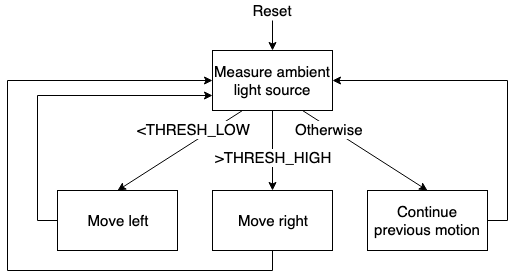
\includegraphics[scale=0.5]{images/move_towards_light_algorithm}
    \caption{Flowchart for move towards light algorithm}
    \label{fig:move_towards_light_algorithm}
\end{figure}
Abovementioned algorithm will help us understand why the robot approaches the source of light in a zig zag fashion. We cannot do significant improvement in algorithm given the limitation of onboard ambient light sensor to one.
\subsection{Demonstration}
Link to the working demo of problem statement can be accessed using link in Figure \ref{fig:move_towards_the_light}.
\begin{figure}[H]
	\centering
	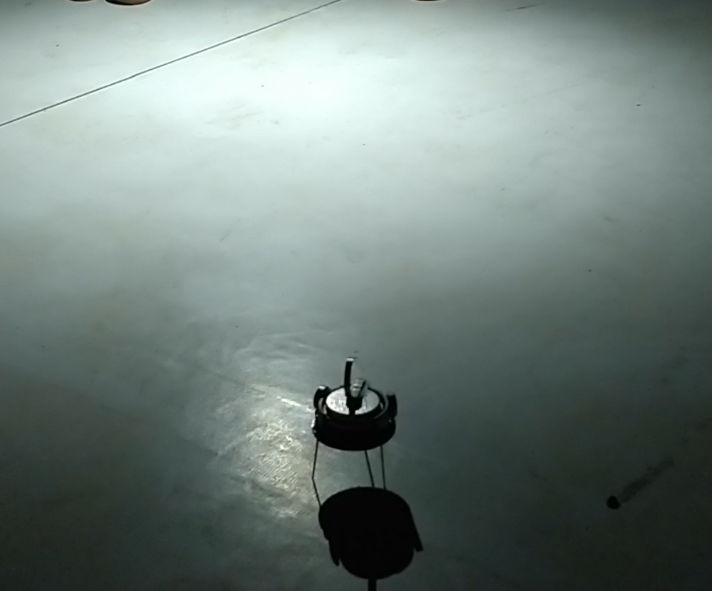
\includegraphics[scale=0.4]{images/move_towards_light}
	\caption{\href{https://www.google.com/url?sa=j&url=https\%3A\%2F\%2Fphotos.app.goo.gl\%2FnUNghDg4nJygpzUu5&uct=1551610784&usg=G0tZGJ7iMN79F5qGk1QMw5rfodM.}{Move towards the light source [Video link]}}
    \label{fig:move_towards_the_light}
\end{figure}
Different $THRESH\_LOW$ and $THRESH\_HI$ parameters were chosen to implement hysteresis behaviour, thereby, precludingjittery motion.

\section{Synchronizing phase of blinking LEDs}
\textbf{Objective}: Create a logical synchronous clock between different 
robots to allow two or more robots to blink an LED in unison roughly every 4 seconds.

\section{Reference}
    \printbibliography[heading=none]
\end{document}
